%! TEX root = main.tex
\documentclass[
  12pt,  % font-size
  oneside,  % Format every page equal
  a4paper,  % Paper
  %  ABNTex2 settings. TITLE is uppercase
  chapter=TITLE, 
  section=TITLE,
  subsection=TITLE,
  subsubsection=TITLE,
  % Babel settings
  english,
  brazil,
  standalone
]{abntex2}

%------------------------------
\usepackage{setup/setup}
%\settocdepth{section}
% ---
%   Bibliography setting
% ---
\usepackage[backend = biber, style=numeric-comp, hyperref]{biblatex}  % style=numeric-comp for numeric style
\setlength\bibitemsep{\baselineskip}
\DeclareFieldFormat{url}{Disponível~em:\addspace\url{#1}}
\NewBibliographyString{sineloco}
\NewBibliographyString{sinenomine}
\DefineBibliographyStrings{brazil}{%
	sineloco     = {\mkbibemph{S\adddot l\adddot}},
	sinenomine   = {\mkbibemph{s\adddot n\adddot}},
	andothers    = {\mkbibemph{et\addabbrvspace al\adddot}},
	in			 = {\mkbibemph{In:}}
}

\addbibresource{aftertext/references.bib}
% Custom citation style to make both name and date appear in blue
\usepackage{xcolor}

\DeclareSourcemap{
  \maps[datatype=bibtex]{
    \map{
      \step[fieldset=abstract, null]
      \step[fieldset=pagetotal, null]
    }
    \map{
      \pertype{inproceedings}
			\step[fieldset=venue, null]
			\step[fieldset=eventdate, null]
			\step[fieldset=eventtitle, null]
			\step[fieldset=isbn, null]
			\step[fieldset=volume, null]
    }
  }
}






% ---
%   Cover informations
% ---

\autor{Rafael Haas Ferracini}

\titulo{Título aqui}

\subtitulo{Subtitulo aqui}

\orientador{Orientador}
%\orientador[Orientadora]{Prof. XXXXX, Dra.}

\coorientador{}
%\coorientador[Orientadora]{Prof. XXXX, Dra.}

\coordenador{}
%\coodernador[Coordenadora]{Prof. XXXX, Dra.}

\ano{2024}
\data{\today}

\local{Florianópolis - SC}

\instituicaosigla{UFSC}
\instituicao{Universidade Federal de Santa Catarina}

\tipotrabalho{Relatório Final}

\formacao{}

\nivel{}

\programa{Programa Institucional de Iniciação Científica e Tecnológica (PIBIC)}

\centro{Campus Florianópolis Departamento de Física}

\preambulo
{%
\imprimirtipotrabalho~do~\imprimirprograma.
}

%------------------------------


% ---
%   PDF settings
% ---
\definecolor{blue}{RGB}{41,5,195}
\makeatletter
\hypersetup{
		pdftitle={\@title}, 
		pdfauthor={\@author},
    pdfsubject={\imprimirpreambulo},
    pdfcreator={LaTeX with abnTeX2},
		pdfkeywords={ufsc, latex, abntex2}, 
		colorlinks=true,
    linkcolor=black,
    citecolor=blue,
    filecolor=blue,
		urlcolor=black,
		bookmarksdepth=4
}
\makeatother

% Declaração das siglas
\siglalista{SIGLAS}{Significado da sigla}

% compila a lista de abreviaturas e siglas e a lista de símbolos
\makenoidxglossaries 

% Compile index
\makeindex

%------------------------------

%%%%%%%%%%%%%%%% DOCUMENT STARTS HERE %%%%%%%%%%%%%%%%
\usepackage[portuguese,onelanguage,ruled,vlined]{algorithm2e}
\begin{document}
  \selectlanguage{brazil}
  \frenchspacing
  \OnehalfSpacing


  % ---
  %   ELEMENTOS PRÉ-TEXTUAIS
  % ---
  %   Capa, folha de rosto, ficha bibliografica, errata, folha de aprovação, dedicatória, agradecimentos, epígrafe, resumos, lista
  % Capa
\imprimircapa


% Folha de Rosto
\imprimirfolhaderosto

% Resumo em Português 
\setlength{\absparsep}{18pt} % ajusta o espaçamento dos parágrafos do resumo
\begin{resumo}
    \SingleSpacing
    AA
    \textbf{Palavras-chave}: Nanomateriais. Cristalografia. Mecanoquímica. 
\end{resumo}

% Resumo em Inglês 
%\begin{resumo}[Abstract]
%	\SingleSpacing
%	\begin{otherlanguage*}{english}
%		Resumo traduzido para outros idiomas, neste caso, inglês. Segue o formato do resumo feito na língua vernácula. As palavras-chave traduzidas, versão em língua estrangeira, são colocadas abaixo do texto precedidas pela expressão “Keywords”, separadas por ponto.
%		
%		\textbf{Keywords}: Keyword 1. Keyword 2. Keyword 3.
%	\end{otherlanguage*}
%\end{resumo}

{%hidelinks
	\hypersetup{hidelinks}
 
	\imprimirlistadesiglas
        
	% inserir o sumario
	\pdfbookmark[0]{\contentsname}{toc}
	\tableofcontents*
	\cleardoublepage
	
}%hidelinks


  % ---
  %   ELEMENTOS TEXTUAIS
  % ---
  \textual

  % 1. Introdução
  
  \chapter{introdução}

\section{Inserir figuras}

\begin{figure}[htb]
  \caption{\label{fig:teste} Figura de teste}
  \centering
  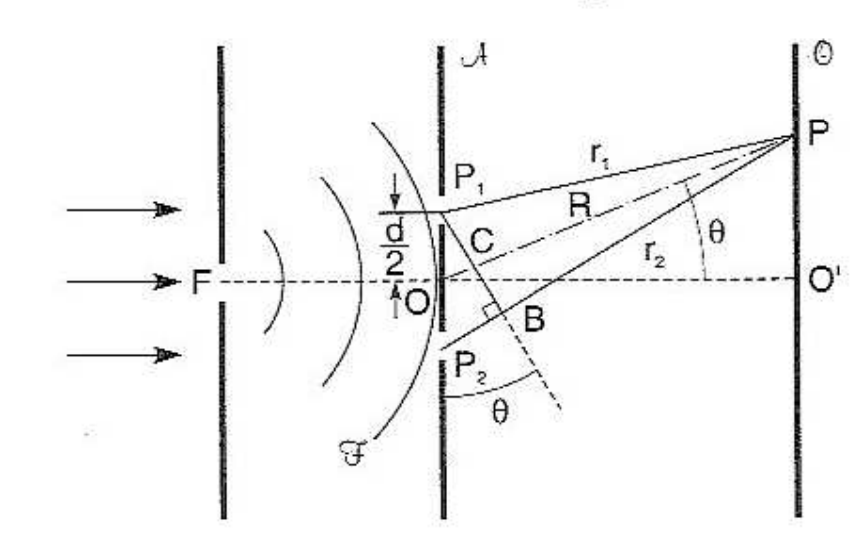
\includegraphics[width=0.8\textwidth]{images/teste.png}
  \fonte{Bota a fonte aqui}
\end{figure}

\section{Lista de Siglas}
Importante definir as siglas em main.tex  na seção "Declaração de Siglas" da seguinte forma:

%\siglalista{SIGLAS}{Significado da sigla}

Quando for fazer menção a sigla, basta usar \gls{SIGLAS}

\section{Coisas úteis}

\emph{Text} Para referenciar a termos estrangeuris (coisas que geralmente colocaria em itálico) \cite{moyses2}
\nocite{halliday4}

Para equações, tabelas e figuras, \autoref{fig:teste} e para nota de rodapé \footnote{É isso ai}




  \include{chapters/2-revisao-bibliografica}
  \include{chapters/3-materiais-e-metodos}
  \include{chapters/4-resultados}
  \chapter{Conclusão}


  
  % ---
  %   ELEMENTOS PÓS-TEXTUAIS
  % ---
  \postextual

  % Referências bibliograficas
  \begingroup
    \SingleSpacing\printbibliography[title=REFERÊNCIAS]
  \endgroup

  % Glossário
  %\glossary

  % Apendices
  %\begin{apendicesenv}
  %  \chapter{Descrição}


Textos elaborados pelo autor, a fim de completar a sua argumentação. Deve ser precedido da palavra APÊNDICE, identificada por letras maiúsculas consecutivas, travessão e pelo respectivo título. Utilizam-se letras maiúsculas dobradas quando esgotadas as letras do alfabeto. 

\begin{quadro}[htb]
	\centering
	\caption{\label{qua:Quadro_2}Modelo A.}	
\begin{tabular}{|l|l|}
\hline
xxxx              & yyyyyyyyyyyyyyy    \\
\hline
xxxx              & yyyyyyyyyyyyyyy    \\
\hline
xxxx              & yyyyyyyyyyyyyyy    \\
\hline
xxxx              & yyyyyyyyyyyyyyy    \\
\hline
xxxx              & yyyyyyyyyyyyyyy    \\
\hline
xxxx              & yyyyyyyyyyyyyyy    \\
\hline
xxxx              & yyyyyyyyyyyyyyy    \\
\hline
rrrrrrrrrrrrrrrrr & eeeeeeeeeeeeeeeee  \\
\hline
xxxx              & yyyyyyyyyyyyyyy    \\
\hline
xxxx              & yyyyyyyyyyyyyyy    \\
\hline
rrrrrrrrrrrrrrrrr & eeeeeeeeeeeeeeeee  \\
\hline
xxxx              & yyyyyyyyyyyyyyy    \\
\hline
                  & ttttttttttttttttt  \\
\hline
rrrrrrrrrrrrrrrrr & eeeeeeeeeeeeeeeee  \\
\hline
ttttttttttttt     &                    \\
\hline
rrrrrrrrrrrrrrrrr & eeeeeeeeeeeeeeeee  \\
\hline
rrrrrrrrrrrrrrrrr & eeeeeeeeeeeeeeeee  \\
\hline
                  & gggggggggggggggggg \\
\hline
rrrrrrrrrrrrrrrrr & eeeeeeeeeeeeeeeee  \\
\hline
rrrrrrrrrrrrrrrrr & eeeeeeeeeeeeeeeee  \\
\hline
rrrrrrrrrrrrrrrrr & eeeeeeeeeeeeeeeee  \\
\hline
rrrrrrrrrrrrrrrrr & eeeeeeeeeeeeeeeee  \\
\hline
\end{tabular}
\fonte{Elaborada pelo autor (2016).}
\end{quadro}

  %\end{apendicesenv}

  % Anexos
  %\begin{anexosenv}
  %  \chapter{Descrição}

São documentos não elaborados pelo autor que servem como fundamentação (mapas, leis, estatutos). Deve ser precedido da palavra ANEXO, identificada por letras maiúsculas consecutivas, travessão e pelo respectivo título. Utilizam-se letras maiúsculas dobradas quando esgotadas as letras do alfabeto.

  %\end{anexosenv}

  % Indice Remissivo
  %\phantompart
  %\printindex

\end{document}
